% !TeX program = pdfLaTeX
\documentclass[12pt]{article}
\usepackage{amsmath}
\usepackage{graphicx,psfrag,epsf}
\usepackage{enumerate}
\usepackage{natbib}
\usepackage{textcomp}
\usepackage[hyphens]{url} % not crucial - just used below for the URL
\usepackage{hyperref}

%\pdfminorversion=4
% NOTE: To produce blinded version, replace "0" with "1" below.
\newcommand{\blind}{0}

% DON'T change margins - should be 1 inch all around.
\addtolength{\oddsidemargin}{-.5in}%
\addtolength{\evensidemargin}{-.5in}%
\addtolength{\textwidth}{1in}%
\addtolength{\textheight}{1.3in}%
\addtolength{\topmargin}{-.8in}%

%% load any required packages here


% Pandoc syntax highlighting
\usepackage{color}
\usepackage{fancyvrb}
\newcommand{\VerbBar}{|}
\newcommand{\VERB}{\Verb[commandchars=\\\{\}]}
\DefineVerbatimEnvironment{Highlighting}{Verbatim}{commandchars=\\\{\}}
% Add ',fontsize=\small' for more characters per line
\usepackage{framed}
\definecolor{shadecolor}{RGB}{248,248,248}
\newenvironment{Shaded}{\begin{snugshade}}{\end{snugshade}}
\newcommand{\AlertTok}[1]{\textcolor[rgb]{0.94,0.16,0.16}{#1}}
\newcommand{\AnnotationTok}[1]{\textcolor[rgb]{0.56,0.35,0.01}{\textbf{\textit{#1}}}}
\newcommand{\AttributeTok}[1]{\textcolor[rgb]{0.77,0.63,0.00}{#1}}
\newcommand{\BaseNTok}[1]{\textcolor[rgb]{0.00,0.00,0.81}{#1}}
\newcommand{\BuiltInTok}[1]{#1}
\newcommand{\CharTok}[1]{\textcolor[rgb]{0.31,0.60,0.02}{#1}}
\newcommand{\CommentTok}[1]{\textcolor[rgb]{0.56,0.35,0.01}{\textit{#1}}}
\newcommand{\CommentVarTok}[1]{\textcolor[rgb]{0.56,0.35,0.01}{\textbf{\textit{#1}}}}
\newcommand{\ConstantTok}[1]{\textcolor[rgb]{0.00,0.00,0.00}{#1}}
\newcommand{\ControlFlowTok}[1]{\textcolor[rgb]{0.13,0.29,0.53}{\textbf{#1}}}
\newcommand{\DataTypeTok}[1]{\textcolor[rgb]{0.13,0.29,0.53}{#1}}
\newcommand{\DecValTok}[1]{\textcolor[rgb]{0.00,0.00,0.81}{#1}}
\newcommand{\DocumentationTok}[1]{\textcolor[rgb]{0.56,0.35,0.01}{\textbf{\textit{#1}}}}
\newcommand{\ErrorTok}[1]{\textcolor[rgb]{0.64,0.00,0.00}{\textbf{#1}}}
\newcommand{\ExtensionTok}[1]{#1}
\newcommand{\FloatTok}[1]{\textcolor[rgb]{0.00,0.00,0.81}{#1}}
\newcommand{\FunctionTok}[1]{\textcolor[rgb]{0.00,0.00,0.00}{#1}}
\newcommand{\ImportTok}[1]{#1}
\newcommand{\InformationTok}[1]{\textcolor[rgb]{0.56,0.35,0.01}{\textbf{\textit{#1}}}}
\newcommand{\KeywordTok}[1]{\textcolor[rgb]{0.13,0.29,0.53}{\textbf{#1}}}
\newcommand{\NormalTok}[1]{#1}
\newcommand{\OperatorTok}[1]{\textcolor[rgb]{0.81,0.36,0.00}{\textbf{#1}}}
\newcommand{\OtherTok}[1]{\textcolor[rgb]{0.56,0.35,0.01}{#1}}
\newcommand{\PreprocessorTok}[1]{\textcolor[rgb]{0.56,0.35,0.01}{\textit{#1}}}
\newcommand{\RegionMarkerTok}[1]{#1}
\newcommand{\SpecialCharTok}[1]{\textcolor[rgb]{0.00,0.00,0.00}{#1}}
\newcommand{\SpecialStringTok}[1]{\textcolor[rgb]{0.31,0.60,0.02}{#1}}
\newcommand{\StringTok}[1]{\textcolor[rgb]{0.31,0.60,0.02}{#1}}
\newcommand{\VariableTok}[1]{\textcolor[rgb]{0.00,0.00,0.00}{#1}}
\newcommand{\VerbatimStringTok}[1]{\textcolor[rgb]{0.31,0.60,0.02}{#1}}
\newcommand{\WarningTok}[1]{\textcolor[rgb]{0.56,0.35,0.01}{\textbf{\textit{#1}}}}

% tightlist command for lists without linebreak
\providecommand{\tightlist}{%
  \setlength{\itemsep}{0pt}\setlength{\parskip}{0pt}}



\usepackage{booktabs}
\usepackage{longtable}
\usepackage{array}
\usepackage{multirow}
\usepackage{wrapfig}
\usepackage{float}
\usepackage{colortbl}
\usepackage{pdflscape}
\usepackage{tabu}
\usepackage{threeparttable}
\usepackage{threeparttablex}
\usepackage[normalem]{ulem}
\usepackage{makecell}
\usepackage{xcolor}

\begin{document}


\def\spacingset#1{\renewcommand{\baselinestretch}%
{#1}\small\normalsize} \spacingset{1}


%%%%%%%%%%%%%%%%%%%%%%%%%%%%%%%%%%%%%%%%%%%%%%%%%%%%%%%%%%%%%%%%%%%%%%%%%%%%%%

\if0\blind
{
  \title{\bf Title here}

  \author{
        Justin Papagelis \thanks{The authors gratefully acknowledge
\ldots{}} \\
    Department of Mathematics and Statistics, Amherst College\\
      }
  \maketitle
} \fi

\if1\blind
{
  \bigskip
  \bigskip
  \bigskip
  \begin{center}
    {\LARGE\bf Title here}
  \end{center}
  \medskip
} \fi

\bigskip
\begin{abstract}
For my project, I plan to explore different bootstrap methods for
creating confidence intervals and then perform comparisons between a
couple of the methods. My paper will re-introduce the idea of bootstrap
to my peers and give some background on constructing confidence
intervals. We will also go deeper into the theory behind the
construction of confidence intervals from bootstrapped data. These
various methods to create a confidence interval from a bootstrap can
include the percentile method, bias-corrected method, accelerated
method, and the studentized method, as well as others. I will
demonstrate how these bootstrap methods work using ``toy examples,''
which will be datasets in which a specific bootstrap method is
appropriate. To demonstrate my understanding of the methods, I will
write a simulation to compare a few of them and determine how they
perform against each other. I will show my understanding of the
different methods of creating confidence intervals from bootstrapped
data by communicating the statistical theory in a concise and accessible
way to my peers. Writing the simulation and sharing conclusions will
demonstrate my ability to implement statistical methods in practice as
well as my ability to analyze the results of the simulation.
\end{abstract}

\noindent%
{\it Keywords:} 3 to 6 keywords, that do not appear in the title
\vfill

\newpage
\spacingset{1.45} % DON'T change the spacing!

\hypertarget{introduction}{%
\section{Introduction}\label{introduction}}

This template will be used for you to submit your final project. You'll
need to install the \emph{rticles} package, make sure you have the
agsm.bst file and bibliography.bib file, and the gfx folder and figure
file in order to compile. If you make your own bibliography.bib file
later, that's fine - change the name above to match your file name.
You'll want the setup for the file to look the same in your repo as in
the class repo, and then compile to asa\_article when you knit. You
should change the name of the file to something other than ``test''
though. Remember that if something goes wrong with the file, you can
always look back at the class repo for the original files and their
structure.

This template was adapted from the template Prof.~Horton provided Stat
495 in Fall 2021, used with permission.

\hypertarget{exposition}{%
\section{Exposition}\label{exposition}}

The portion of the paper where you describe the new technique as though
you were teaching it to a classmate (with whatever name you want to give
it - Literature, Background, or Exposition) will be based on your
annotated bibliography. You can add sources to what you already have in
the annotated bibliography (especially if my feedback says you need
to!). To be sure that you are on track with the exposition, a full draft
of this portion of the paper is due before Thanksgiving break. This will
also help with incorporating proper citation early in the writing
process, as you'll have a bibliography that we can implement for this
portion of the paper at a minimum.

Exposition -\textgreater{} what is a bootstrap --\textgreater{}
parametric --\textgreater{} non-parametric --\textgreater{} briefly:
what is jackknife nah --\textgreater{} SE and bias? -\textgreater{} what
is a bootstrapped confidence interval --\textgreater{} what can it do
-\textgreater{} how do we create them -\textgreater{} different types of
bootstrapped CI --\textgreater{} standard t interval, approx classical,
swapped SE, percentile, Bias-corrected, BCa ---\textgreater{} for sample
mean or corr (check example sheet)

Bootstrapping is a statistical method of resampling that allows the
estimation of a test statistic from an unknown distribution. In
particular, bootstrapping is a computational heavy method which is
useful for many different situations.

First, we will introduce the non-parametric bootstrap. Suppose we have a
random sample \(X = (x_1,x_2,\dots,x_n)\) from our unknown distribution,
\(F\) and a statistic of interest \(\hat{\theta} = \hat{\theta}(X)\).
Ideally, the desired test statistic could be found by repeatedly
sampling new reproductions of \(X\) from \(F\). However \(F\) is unknown
so this is not possible. The non-parametric bootstrap creates an
estimate \(\hat{F}\) from \(F\) using our sample \(X\) without making
any parametric assumptions (such as distribution). Therefore, the
bootstrap sample could be represented as
\(X^* = (x^*_1, x^*_2, \dots, x^*_n)\) where each \(x^*_i\) is sampled
randomly with equal probability and with replacement from
\(\{x_1,x_2,\dots,x_n\}\). From this bootstrap sample, a bootstrap
replication of the test statistic can be computed using
\(\hat{\theta}^* = \hat{\theta}(X^*)\). A large number, \(B\), of
bootstrap samples are drawn independently and the corresponding
bootstrap replication of the test statistic is calculated.
\[\hat{\theta}^{*b} = \hat{\theta}(X^{*b}) \text{ for } b = 1,2, \dots, B\].
The bootstrap estimate of the test statistic is the empirical value of
the test statistic from all of the \(\hat{\theta}^{*b}\) replications.
As \(B\) increases, \(\hat{F}\) approaches \(F\) which means that the
tests statistic of interest approaches its true value as well.

SHOULD I ADD ABOUT PARAMETRIC BOOTSTRAP

Confidence intervals are tools that are used to estimate a parameter.
Specifically, a confidence interval gives a range in which the true
value of the parameter may lie. An \(\alpha\)-level standard confidence
interval is given by \[\hat{\theta} \pm z_{\alpha}\hat{\sigma}\] where
\(\hat{\theta}\) is a point estimate of the parameter of interest
\(\theta\), \(\hat{\sigma}\) is the estimate of the standard deviation
of \(\hat{\theta}\) and \(z_{\alpha}\) is the \((100 *\alpha)\)th
percentile of the normal deviation. We say that the confidence interval
constructed in this manner has a chance of capturing the true parameter
with a probability of \(\alpha\).

The standard confidence interval is built based on the assumption that
the distribution from which we are sampling is Normal. This means that
for an unknown distribution, the standard confidence interval could
present an incorrect range. However, the same process can be used with
bootstrap sampling to form the bootstrap percentile method. This means
that an approximate bootstrap confidence interval will be created in the
same automatic way that the standard confidence interval was created.

The percentile method interval is defined as the interval between the
\(100 * \alpha\) and the \(100(1 - \alpha)\) percentiles of the
bootstrap distribution of \(\hat{\theta}\). That is, the
\((1 - 2\alpha)\) coverage interval can be defined as
\[[\hat{\theta}^*_\alpha,\hat{\theta}^*_{1-\alpha}].\] In the case that
the bootstrap distribution of
\(\hat{\theta}^* \sim N(\hat{\theta}, \hat{\sigma}^2)\), the
corresponding percentile interval would be equivalent to the standard
interval. However, this is not usually the case. When the bootstrap
distribution is non-normal, we can suppose that there exists, for all
\(\theta\), \[\hat{\phi} \sim N(\phi, \tau^2),\] for some monotone
transformation \(\hat{\phi} = g(\hat{\theta}), \phi = g(\theta)\), and
\(\tau\) is a constant. In other words, this transformation perfectly
normalizes the distribution of \(\hat{\theta}\). This transformation
invariant can be applied to the bootstrap replications such that
\[\hat{\phi}^{*b} = g\left( \hat{\theta}^{*b}\right ) \text{ for } b = 1,2,\dots, B.\]
The corresponding percentiles of the distribution transform similarly,
\(\hat{\phi}^*_\alpha = g \left ( \hat{\theta}^*_\alpha \right )\). Or
we can say that the \((1 - 2\alpha)\) percentile interval is
\(\hat{\phi} \pm \tau z_\alpha\) which can also be represented as
\([\hat{\phi}^*_\alpha,\hat{\phi}^*_{1-\alpha}]\). This means that the
interval on the \(\theta\) scale can be defined as
\[\hat{\theta}^*_\alpha = g^{-1}(\hat{\phi} \pm \tau z_\alpha).\] Or
\(\left [ g^{-1}(\hat{\phi} \pm \tau z_{1-\alpha}), g^{-1}(\hat{\phi} \pm \tau z_\alpha) \right ]\).
Therefore, the percentile method produces a correct interval for
\(\phi\) and due to the transformation invariance, also produces a
correct percentile interval for \(\theta\). This method assumes the
existence of some monotone normalizing mapping
\(\hat{\phi} = g(\hat{\theta}), \phi = g(\theta)\) and relies on that to
create a correct interval. Since the process is automatic, we do not
need to know the transformation itself, only that it exists. However, in
some cases, no monotone normalizing mapping will exist.

\hypertarget{more-on-the-template}{%
\section{More on the template}\label{more-on-the-template}}

\label{sec:template}

This template demonstrates some of the basic LaTeX commands and syntax
you'll need to know to use the \texttt{rticles} package to generate a
readable report using R Markdown. Markdown allows various formatting and
you can find formatting cheatsheets or guides online to assist as well.
Here's an example with bullets and some advice:

\begin{itemize}
\tightlist
\item
  I would encourage you to look closely at this file and explore the
  various parts and pieces.
\item
  I would suggest that you format your Rmd file so that you have only
  one sentence per line.
\item
  It makes it \emph{much} easier to see changes in your GitHub commits.
\end{itemize}

\section{Verifications}
\label{sec:verify}

This section will be just long enough to illustrate what a full page of
text looks like, for margins and spacing.

Note that we can refer to sections (e.g., this is section
\ref{sec:verify}, while the previous section was section
\ref{sec:template}).

Note that we should refer to work using the BibTeX system. Here we can
reference papers by \citet{Campbell02} and \citet{Schubert13} through
inline citations (see the \texttt{bibliography.bib} file for the
reference database).

More work that is relevant can also be cited in a traditional fashion
\citep[\citet{Galyardt14mmm},\citet{Galyardt12dis}]{Chi81}.

Note that you can capitalize proper nouns in citations
\citep{Campbell02} (again, see \texttt{bibliography.bib}).

The quick brown fox jumped over the lazy dog. The quick brown fox jumped
over the lazy dog. The quick brown fox jumped over the lazy dog. The
quick brown fox jumped over the lazy dog. \textbf{With this spacing we
have 30 lines per page.}

The quick brown fox jumped over the lazy dog. The quick brown fox jumped
over the lazy dog. The quick brown fox jumped over the lazy dog. The
quick brown fox jumped over the lazy dog. The quick brown fox jumped
over the lazy dog.

The quick brown fox jumped over the lazy dog. The quick brown fox jumped
over the lazy dog. The quick brown fox jumped over the lazy dog. The
quick brown fox jumped over the lazy dog. The quick brown fox jumped
over the lazy dog. The quick brown fox jumped over the lazy dog. The
quick brown fox jumped over the lazy dog. The quick brown fox jumped
over the lazy dog. The quick brown fox jumped over the lazy dog. The
quick brown fox jumped over the lazy dog.

The quick brown fox jumped over the lazy dog. The quick brown fox jumped
over the lazy dog. The quick brown fox jumped over the lazy dog. The
quick brown fox jumped over the lazy dog. The quick brown fox jumped
over the lazy dog. The quick brown fox jumped over the lazy dog. The
quick brown fox jumped over the lazy dog. The quick brown fox jumped
over the lazy dog. The quick brown fox jumped over the lazy dog. The
quick brown fox jumped over the lazy dog.

The quick brown fox jumped over the lazy dog. The quick brown fox jumped
over the lazy dog. The quick brown fox jumped over the lazy dog. The
quick brown fox jumped over the lazy dog. The quick brown fox jumped
over the lazy dog. The quick brown fox jumped over the lazy dog. The
quick brown fox jumped over the lazy dog. The quick brown fox jumped
over the lazy dog. The quick brown fox jumped over the lazy dog. The
quick brown fox jumped over the lazy dog.

The quick brown fox jumped over the lazy dog. The quick brown fox jumped
over the lazy dog. The quick brown fox jumped over the lazy dog. The
quick brown fox jumped over the lazy dog. The quick brown fox jumped
over the lazy dog. The quick brown fox jumped over the lazy dog. The
quick brown fox jumped over the lazy dog. The quick brown fox jumped
over the lazy dog. The quick brown fox jumped over the lazy dog. The
quick brown fox jumped over the lazy dog.

The quick brown fox jumped over the lazy dog. The quick brown fox jumped
over the lazy dog. The quick brown fox jumped over the lazy dog. The
quick brown fox jumped over the lazy dog. The quick brown fox jumped
over the lazy dog. The quick brown fox jumped over the lazy dog. The
quick brown fox jumped over the lazy dog. The quick brown fox jumped
over the lazy dog. The quick brown fox jumped over the lazy dog. The
quick brown fox jumped over the lazy dog.

The quick brown fox jumped over the lazy dog. The quick brown fox jumped
over the lazy dog. The quick brown fox jumped over the lazy dog. The
quick brown fox jumped over the lazy dog. The quick brown fox jumped
over the lazy dog. The quick brown fox jumped over the lazy dog. The
quick brown fox jumped over the lazy dog. The quick brown fox jumped
over the lazy dog. The quick brown fox jumped over the lazy dog. The
quick brown fox jumped over the lazy dog.

The quick brown fox jumped over the lazy dog. The quick brown fox jumped
over the lazy dog. The quick brown fox jumped over the lazy dog. The
quick brown fox jumped over the lazy dog. The quick brown fox jumped
over the lazy dog. The quick brown fox jumped over the lazy dog. The
quick brown fox jumped over the lazy dog. The quick brown fox jumped
over the lazy dog. The quick brown fox jumped over the lazy dog. The
quick brown fox jumped over the lazy dog.

The quick brown fox jumped over the lazy dog. The quick brown fox jumped
over the lazy dog. The quick brown fox jumped over the lazy dog. The
quick brown fox jumped over the lazy dog. The quick brown fox jumped
over the lazy dog. The quick brown fox jumped over the lazy dog. The
quick brown fox jumped over the lazy dog. The quick brown fox jumped
over the lazy dog. The quick brown fox jumped over the lazy dog. The
quick brown fox jumped over the lazy dog.

\hypertarget{examples}{%
\section{Examples}\label{examples}}

Lots of things can be done in this template.

\begin{Shaded}
\begin{Highlighting}[]
\NormalTok{Violations }\SpecialCharTok{\%\textgreater{}\%}
  \FunctionTok{select}\NormalTok{(dba, boro) }\SpecialCharTok{\%\textgreater{}\%}
  \FunctionTok{unique}\NormalTok{() }\SpecialCharTok{\%\textgreater{}\%}
  \FunctionTok{group\_by}\NormalTok{(boro) }\SpecialCharTok{\%\textgreater{}\%}
  \FunctionTok{summarize}\NormalTok{(}\AttributeTok{count =} \FunctionTok{n}\NormalTok{(), }\AttributeTok{.groups =} \StringTok{"drop"}\NormalTok{) }\SpecialCharTok{\%\textgreater{}\%}
\NormalTok{  knitr}\SpecialCharTok{::}\FunctionTok{kable}\NormalTok{(}
    \AttributeTok{caption =} \StringTok{"This is a sample table caption that should interpret the table!"}\NormalTok{)}
\end{Highlighting}
\end{Shaded}

\begin{table}

\caption{\label{tab:sample-table1}This is a sample table caption that should interpret the table!}
\centering
\begin{tabular}[t]{l|r}
\hline
boro & count\\
\hline
BRONX & 1903\\
\hline
BROOKLYN & 5294\\
\hline
MANHATTAN & 8340\\
\hline
Missing & 6\\
\hline
QUEENS & 4789\\
\hline
STATEN ISLAND & 802\\
\hline
\end{tabular}
\end{table}

Table \ref{tab:sample-table1} displays the number of dba's per borough.

\begin{Shaded}
\begin{Highlighting}[]
\NormalTok{Violations }\SpecialCharTok{\%\textgreater{}\%}
  \FunctionTok{select}\NormalTok{(dba, boro, inspection\_date, score) }\SpecialCharTok{\%\textgreater{}\%}
  \FunctionTok{unique}\NormalTok{() }\SpecialCharTok{\%\textgreater{}\%}
  \FunctionTok{group\_by}\NormalTok{(boro) }\SpecialCharTok{\%\textgreater{}\%}
  \FunctionTok{summarize}\NormalTok{(}
    \AttributeTok{count =} \FunctionTok{n}\NormalTok{(),}
    \AttributeTok{averagescore =} \FunctionTok{mean}\NormalTok{(score, }\AttributeTok{na.rm =} \ConstantTok{TRUE}\NormalTok{),}
    \AttributeTok{.groups =} \StringTok{"drop"}
\NormalTok{  ) }\SpecialCharTok{\%\textgreater{}\%}
  \FunctionTok{ggplot}\NormalTok{(}\FunctionTok{aes}\NormalTok{(}\AttributeTok{x =}\NormalTok{ boro, }\AttributeTok{y =}\NormalTok{ averagescore)) }\SpecialCharTok{+}
  \FunctionTok{geom\_boxplot}\NormalTok{()}
\end{Highlighting}
\end{Shaded}

\begin{figure}
\centering
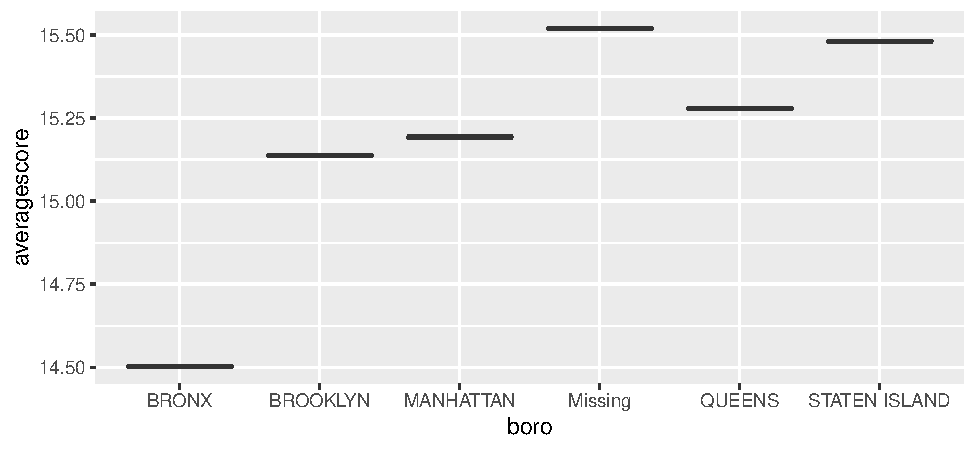
\includegraphics{paper_files/figure-latex/sample-fig1-1.pdf}
\caption{\label{fig:sample-fig1}This is a sample figure caption that
should interpret the figure!}
\end{figure}

Figure \ref{fig:sample-fig1} displays the average inspection score by
borough.

Figure \ref{fig:sample-fig2} displays a campus map.

\begin{figure}
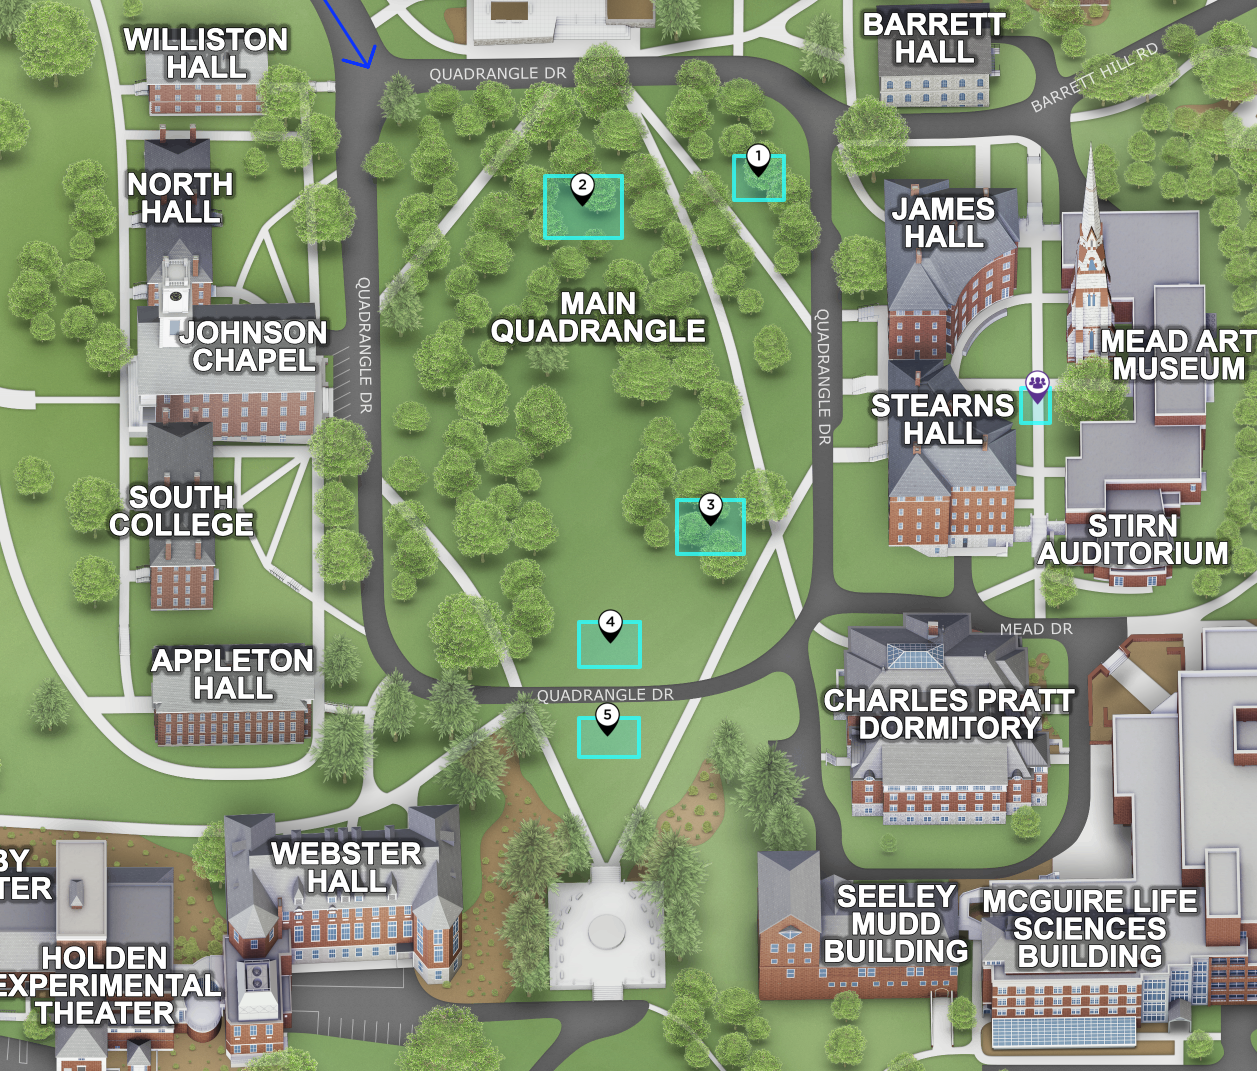
\includegraphics[width=0.8\linewidth]{gfx/campus_map} \caption{XX another sample figure caption}\label{fig:sample-fig2}
\end{figure}

The quick brown fox jumped over the lazy dog. The quick brown fox jumped
over the lazy dog. The quick brown fox jumped over the lazy dog. The
quick brown fox jumped over the lazy dog. The quick brown fox jumped
over the lazy dog. The quick brown fox jumped over the lazy dog. The
quick brown fox jumped over the lazy dog. The quick brown fox jumped
over the lazy dog. The quick brown fox jumped over the lazy dog. The
quick brown fox jumped over the lazy dog.

The quick brown fox jumped over the lazy dog. The quick brown fox jumped
over the lazy dog. The quick brown fox jumped over the lazy dog. The
quick brown fox jumped over the lazy dog.

\hypertarget{your-choice-of-structure}{%
\section{Your Choice of Structure}\label{your-choice-of-structure}}

You are responsible for choosing the structure you want for the report,
i.e.~what sections and their names. Here are some examples that you
could adapt, as appropriate. These are just examples - the first has
more sections, some of which may make more sense as sub-sections of
others. I'm just trying to give you examples. You don't have to have a
conclusion or an introduction, etc. You'll need to find what works for
you.

\hypertarget{example-1}{%
\subsection{Example 1}\label{example-1}}

\begin{itemize}
\tightlist
\item
  Introduction
\item
  Background
\item
  Topic X (Main exposition section)
\item
  Applications in Literature
\item
  Application to Data (your data)
\item
  Conclusion
\end{itemize}

\hypertarget{example-2}{%
\subsection{Example 2}\label{example-2}}

\begin{itemize}
\tightlist
\item
  Introduction (including any relevant Background)
\item
  Topic X (exposition and examples)
\item
  Simulation
\end{itemize}

\bibliographystyle{agsm}
\bibliography{bibliography.bib}


\end{document}
